\chapter{Video Compression using GStreamer}
\label{chap:gstreamer}

\section{Motivation}
A significant amout of work was put into enabling on the fly compression of the videostreams from the \sr.
That is the ability to compress the video data as it is being recorded, and storing the compressed data on disk.

The sensor rig produces roughly 2Gib of data per second with a stereo camera setup.
At this rate it infeasable to record long datasets as almost a terrabyte of data is produced every hour.
\begin{align}
    \frac{1TB}{2Gb/s} & = \frac{8Tb}{2Gb/s}
                      &                     & = 4000s
                      &                     & \approx 1h + 7min
\end{align}

It is reasonable to say that a much easer option is to buy \gls{ssd} with a capacity up to 8TB \cite{CorsairMP600PRO}, enabling roughly 9 hours of recording.
One reason this
\cite{microntechnologyMicron2300SSD2020}


\paragraph{Limited write speed}
One issue when storing the raw data at first was that the \jx was not able to write to the disk fast to the installed \gls{ssd}.
The write speed was tested using:
\begin{minted}[linenos=false]{bash}
    sudo dd if=/dev/zero of=./testfile bs=8k count=100k conv=fdatasync
\end{minted}
which repeatedly reported write speeds just below $2Gb/s$ (250MB).
This is weird, as the \gls{ssd} has a write speed of $2.7GB/s$, but other people have faced similar issues on the \jx \cite{microntechnologyMicron2300SSD2020} \cite{dtyuImbalancedPerformanceRead2018}.
This is probably fixable, but provides further motivation to enable on the fly compression



However, there are three additional reasons on the fly compression is desirable:
If the sensor rig is mounted on a ship, it will be possible to transfer all the data to a storage server on the ship over regular ether net, using the ethernet port on the \jx which is limited to 1Gb/s.

By adjusting the compression rate of the sensor rig data can be transferred over ethernet for remote real time processing.
The compression has to be done at some point anyway.






% \begin{figure}
%     \centering
%     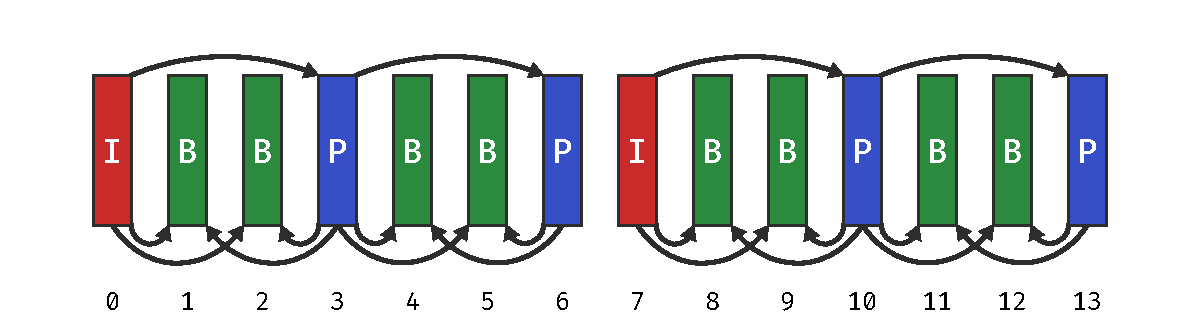
\includegraphics[width=0.8\textwidth]{figures/compression/ipb_frames.webp}
%     \caption{Frames}
%     \label{fig:ipbframes}
% \end{figure}